% !Mode:: "TeX:UTF-8"
% !TEX program  = xelatex

%\documentclass{cumcmthesis}
\documentclass[withoutpreface,bwprint]{cumcmthesis} %去掉封面与编号页

\usepackage{url}   % 网页链接
\usepackage{subcaption} % 子标题
\usepackage{cases}
\title{全国大学生数学建模竞赛编写的 \LaTeX{} 模板}
\tihao{A}
\baominghao{4321}
\schoolname{XX大学}
\membera{}
\memberb{向左}
\memberc{哈哈}
\supervisor{老师}
\yearinput{2017}
\monthinput{08}
\dayinput{22}

\title{一维抛物型方程的差分格式 ~\\ ~\\ \normalsize 肖名财 \quad 刘礼海}
\begin{document}
	\maketitle
	\section{引言}
	在研究热传导过程、气体膨胀过程和电磁场的传播等问题时,常常会遇到抛物型偏微分方程。这类方程的自变量中有一个是实际中的时间变量,用t表示。本文研究一维非齐次热传导方程的Dirichlet初边值问题:
%	\begin{gather}
%	\left\}
%	x^2+y^2=z^2 \label{eq:r2} \\
%	x^3+y^3=z^3 \notag \\
%	x^4+y^4=z^4 \tag{$*$} \\
%	x^5+y^5=z^5 \tag*{$*$} \\
%	x^6+y^6=z^6 \tag{???$'$}
%	\right.
%	\end{gather}
\begin{subequations}
	\begin{numcases}{}
	\dfrac{\partial{u}}{\partial{t}}-a\dfrac{\partial^2{u}}{\partial{x^2}}=f(x,t) , 0 \leq x \leq 1,0 \leq t \leq T \label{1a} \\
	u(x,0)=\varphi(x),0 \leq x \leq 1  \label{1b}\\
	u(0,t)=\alpha(t),u(1,t)=\beta(t),0 \leq t \leq 1 \label{1c}
	\end{numcases}
\end{subequations}

其中$a$为正常数,$f(x,t),\varphi(t),\alpha(t),\beta(t)$为已知函数,$\varphi(0)=\alpha(0),\varphi(1)=\beta(0)$

称(\ref{1b})为初值条件,(\ref{1c})为边值条件。

\section{数值格式}
首先,将区间[0,1]作m等分,将区间[0,T]作n等分,记$h=\dfrac{1}{m},\tau=\dfrac{T}{h}$,$x_i=ih,0 \leq i \leq m,t_k=k\tau,0 \leq k \leq n$

分别称$h$和$\tau$为空间步长和时间步长。

称在t=0,x=0,x=1处的节点为内节点,其他节点为边界节点,称在直线$t=t_k$上的所有节点${(x_i,t_k)|0 \leq i \leq m}$为第$k$层节点。


\subsection{向后Euler格式}
在节点$(x_i,t_k)$处考虑微分方程(\ref{1a}),有
\begin{equation}
\label{e2}
\dfrac{\partial{u}}{\partial{t}}(x_i,t_k)-a\dfrac{\partial^2{u}}{\partial{x^2}}(x_i,t_k)=f(x_i,t_k), 1 \leq i \leq m-1,0 \leq k \leq n-1
\end{equation}

用二阶中心差商代替二阶导数
\begin{equation}
\label{e3}
\dfrac{\partial^2{u}}{\partial{x^2}}(x_i,t_k)=\dfrac{1}{h^2}[u(x_{i-1,t_k})-2u(x_i,t_k)+u(x_{i+1},t_k)]+O(h^2)
\end{equation}

用向后差商代替一阶导数
\begin{equation}
\label{e4}
\dfrac{\partial{u}}{\partial{t}}(x_i,t_k)=\dfrac{u(x_i,t_k)-u(x_i,t_{k-1})}{\tau}+O(\tau)
\end{equation}

将(\ref{e3})和(\ref{e4})带入(\ref{e2})式,得
\begin{equation}
\label{e5}
\dfrac{u(x_i,t_{k})-u(x_i,t_{k-1})}{\tau}-a\dfrac{u(x_{i-1,t_k})-2u(x_i,t_k)+u(x_{i+1},t_k)}{h^2}=f(x_i,t_k)+O(h^2+\tau)
\end{equation}

截断误差为$O(h^2+\tau)$.

在(\ref{e5})中略去截断误差,得差分格式
\begin{subequations}
	\begin{numcases}{}
	\dfrac{u(x_i,t_{k})-u(x_i,t_{k-1})}{\tau}-a\dfrac{u(x_{i-1,t_k})-2u(x_i,t_k)+u(x_{i+1},t_k)}{h^2}=f(x_i,t_k) \label{e6_a} \\
	u_i^0=\varphi(x_i),0 \leq i \leq m \label{e6_b} \\
	u_0^k=\alpha(t_k),u_m^k=\beta(t_k),1\leq k \leq n \label{e6_c}
	\end{numcases}
\end{subequations}
称(\ref{e6_a})-(\ref{e6_c})为向后Euler格式.

记$\gamma=\dfrac{a\tau}{h^2}$,称$\gamma$为步长比,(\ref{e6_a})整理得
\begin{equation}
\label{e7}
-\gamma u_{i-1}^k+(1+2\gamma)u_i^k-\gamma u_{i+1}^k=u_i^{k-1}+\tau f(x_i,t_k),1 \leq i \leq m-1,0 \leq k \leq n-1
\end{equation}

写成矩阵形式
\begin{equation}
\label{e8}
Au=f
\end{equation}

其中
$$
A=
\begin{bmatrix}
1+2\gamma & -\gamma \\
-\gamma & 1+2\gamma & -\gamma \\
& \ddots & \ddots & \ddots \\
& & 	-\gamma & 1+2\gamma
\end{bmatrix}
$$


$$
u=
\begin{bmatrix}
u_1^k\\
u_2^k\\
\vdots\\
u_{m-2}^k \\
u_{m-1}^k
\end{bmatrix}
$$.

$$f=
\begin{bmatrix}
u_1^{k-1}+\gamma u_0^k\\
u_2^{k-1}\\
\vdots\\
u_{m-2}^{k-1} \\
u_{m-1}^{k-1}+\gamma u_m^k
\end{bmatrix}
+
\begin{bmatrix}
\tau f(x_1,t_k)\\
\tau f(x_2,t_k)\\
\vdots\\
\tau f(x_{m-2},t_k) \\
\tau f(x_{m-1},t_k)
\end{bmatrix}
$$.

解方程(\ref{e8}),可以得到数值解。

\subsection{Crank-Nicolson格式}
引入半整数点
记$t_{k+\frac{1}{2}}=\dfrac{1}{2}(t_k+t_{k+1})$

在点$ (x_i,t_{k+\frac{1}{2}}) $处考虑微分方程(\ref{1a}),有
\begin{equation}
\label{e9}
\dfrac{\partial{u}}{\partial{t}}(x_i,t_{k+\frac{1}{2}})-a\dfrac{\partial^2{u}}{\partial{x^2}}(x_i,t_k)=f(x_i,t_{k+\frac{1}{2}}), 1 \leq i \leq m-1,0 \leq k \leq n-1
\end{equation}

由Taylor展开得
\begin{equation}
\label{e10}
\dfrac{\partial^2{u}}{\partial{x}^2}(x_i,t_k)=\dfrac{\partial^2{u}}{\partial{x}^2}(x_i,t_{k+\frac{1}{2}})-\dfrac{\tau}{2}\dfrac{\partial^3{u}}{\partial{x}^2\partial{t}}+\dfrac{1}{2}(\dfrac{\tau}{2})^2\dfrac{\partial^4{u}}{\partial{x}^2\partial{t}^2}+O(\tau^3)
\end{equation}

\begin{equation}
\label{e11}
\dfrac{\partial^2{u}}{\partial{x}^2}(x_i,t_{k+1})=\dfrac{\partial^2{u}}{\partial{x}^2}(x_i,t_{k+\frac{1}{2}})+\dfrac{\tau}{2}\dfrac{\partial^3{u}}{\partial{x}^2\partial{t}}+\dfrac{1}{2}(\dfrac{\tau}{2})^2\dfrac{\partial^4{u}}{\partial{x}^2\partial{t}^2}+O(\tau^3)
\end{equation}

将(\ref{e10})和(\ref{e11})相加得
\begin{equation}
\label{e12}
\dfrac{\partial^2{u}}{\partial{x}^2}(x_i,t_{k+\frac{1}{2}})=\dfrac{1}{2}[\dfrac{\partial^2{u}}{\partial{x}^2}(x_i,t_{k+1})+\dfrac{\partial^2{u}}{\partial{x}^2}(x_i,t_{k})]+O(\tau^2)
\end{equation}

将(\ref{e12})带入(\ref{e9})得
\begin{equation}
\label{e13}
\dfrac{\partial{u}}{\partial{t}}(x_i,t_{k+\frac{1}{2}})-\dfrac{1}{2}a[\dfrac{\partial^2{u}}{\partial{x}^2}(x_i,t_{k+1})+\dfrac{\partial^2{u}}{\partial{x}^2}(x_i,t_{k})]=f(x_i,t_{k+\frac{1}{2}})+O(\tau^2)
\end{equation}

用一阶中心差商近似一阶导数
\begin{equation}
\label{e14}
\dfrac{\partial{u}}{\partial{t}}(x_i,t_{k+\frac{1}{2}})=\dfrac{u(x_i,t_{k+1})-u(x_i,t_k))}{\tau}+O(\tau^2)
\end{equation}

用二阶中心差商近似二阶导数
\begin{equation}
\label{e15}
\dfrac{\partial^2{u}}{\partial{x}^2}(x_i,t_{k})=\dfrac{u(x_{i+1},t_k)-2u(x_i,t_k)+u(x_{i-1},t_k)}{h^2}+O(h^2)
\end{equation}

\begin{equation}
\label{e16}
\dfrac{\partial^2{u}}{\partial{x}^2}(x_i,t_{k+1})=\dfrac{u(x_{i+1},t_{k+1})-2u(x_i,t_{k+1})+u(x_{i-1},t_{k+1})}{h^2}+O(h^2)
\end{equation}

将(\ref{e14})、(\ref{e15})和(\ref{e16})代入(\ref{e13}),得
\begin{equation}
\begin{aligned}
\label{e17}
\dfrac{u(x_i,t_{k+1})-u(x_i,t_k))}{\tau}-\dfrac{a}{2}[\dfrac{u(x_{i+1},t_k)-2u(x_i,t_k)+u(x_{i-1},t_k)}{h^2}+\\
\dfrac{u(x_{i+1},t_{k+1})-2u(x_i,t_{k+1})+u(x_{i-1},t_{k+1})}{h^2}]=f(x_i,t_{k+\frac{1}{2}})+O(h^2+\tau^2)
\end{aligned}
\end{equation}

略去截断误差,从而可得差分方程
\begin{subequations}
	\begin{numcases}{}
	\dfrac{u_i^{k+1}-u_i^k}{\tau}=\dfrac{a}{2}[\dfrac{u_{i+1}^{k}-2u_i^{k}+u_{i-1}^{k}}{h^2}+\dfrac{u_{i+1}^{k+1}-2u_i^{k+1}+u_{i-1}^{k+1}}{h^2}] +f(x_i,t_{k+\frac{1}{2}}) \label{e18_a}\\
	u_i^0=\varphi(x_i),0\leq i \leq m \\
	u_0^k=\alpha(t_k),u_m^k=\beta(t_k),1 \leq k \leq n
	\end{numcases}
\end{subequations}

截断误差为$ O(\tau^2+h^2) $.

将(\ref{e18_a})写成矩阵形式
\begin{equation}
\label{e19}
A_1u^{k+1}=A_2u^k+f
\end{equation}
其中
$$
A_1=
\begin{bmatrix}
1+\gamma & -\dfrac{\gamma}{2} \\
-\dfrac{\gamma}{2} & 1+\gamma & -\dfrac{\gamma}{2} \\
& \ddots & \ddots & \ddots \\
& & 	-\dfrac{\gamma}{2} & 1+\gamma
\end{bmatrix}
$$

$$
A_2=
\begin{bmatrix}
1-\gamma & \dfrac{\gamma}{2} \\
\dfrac{\gamma}{2} & 1-\gamma & \dfrac{\gamma}{2} \\
& \ddots & \ddots & \ddots \\
& & 	\dfrac{\gamma}{2} & 1-\gamma
\end{bmatrix}
$$

$$
u^k=
\begin{bmatrix}
u_1^k\\
u_2^k\\
\vdots\\
u_{m-2}^k \\
u_{m-1}^k
\end{bmatrix}
$$.

$$
f=
\begin{bmatrix}
\dfrac{\gamma}{2}(u_0^k+u_0^{k+1})+\tau f(x_1,t_{k+\frac{1}{2}}) \\
\tau f(x_2,t_{k+\frac{1}{2}})\\
\vdots \\
\tau f(x_{m-2},t_{k+\frac{1}{2}}) \\
\dfrac{\gamma}{2}(u_m^k+u_m^{k+1})+\tau f(x_{m-1},t_{k+\frac{1}{2}})
\end{bmatrix}
$$

解(\ref{e19}),即可得数值解。


\subsection{二阶BDF差分格式}
当k=1时,直接对(\ref{1a})运用向后Euler差分格式,有
\begin{equation}
\label{e20}
\dfrac{u_i^1-u_i^0}{\tau}=a\dfrac{u_{i-1}^1-2u_i^1+u_{i+1}^1}{h^2}+f_i^1 ,1 \leq i \leq m-1
\end{equation}
截断误差$ R=O(h^2+\tau) $


当$ k \geq 2 $时,在点$(x_i,t_k)$处考虑方程(\ref{1a}),有

\begin{equation}
\label{e21}
\dfrac{\partial{u}}{\partial{t}}(x_i,t_k)=a\dfrac{\partial^2{u}}{\partial{t}^2}(x_i,t_k)+f(x_i,t_k)
\end{equation}

将$ u(x_i,t_{k-1}) $,$ u(x_i,t_{k-2}) $在点$ (x_i,t_k) $处Taylor展开,有
\begin{equation}
\label{e22}
u(x_i,t_{k-1})=u(x_i,t_k)-\tau \dfrac{\partial{u}}{\partial{t}}(x_i,t_k)+\dfrac{1}{2!}\tau^2\dfrac{\partial^2{u}}{\partial{t}^2}(x_i,t_k)-\dfrac{1}{3!}\tau^3\dfrac{\partial^3{u}}{\partial{t}^3}(x_i,t_k)+O(\tau^3)
\end{equation}

\begin{equation}
\label{e23}
u(x_i,t_{k-2})=u(x_i,t_k)-2\tau \dfrac{\partial{u}}{\partial{t}}(x_i,t_k)+\dfrac{1}{2!}(2\tau)^2\dfrac{\partial^2{u}}{\partial{t}^2}(x_i,t_k)-\dfrac{1}{3!}(2\tau)^3\dfrac{\partial^3{u}}{\partial{t}^3}(x_i,t_k)+O(\tau^3)
\end{equation}


$ (\ref{e23})-4\times(\ref{e22}) $得
\begin{equation}
\label{e24}
\dfrac{u(x_i,t_{k-2})-4u(x_i,t_{k-1})+3u(x_i,t_k)}{2\tau}=\dfrac{\partial{u}}{\partial{t}}(x_i,t_k)+O(\tau^2)
\end{equation}

用二阶中心差商代替二阶导数
\begin{equation}
\label{e25}
\dfrac{\partial^2{u}}{\partial{x}^2}(x_i,t_{k})=\dfrac{u(x_{i+1},t_k)-2u(x_i,t_k)+u(x_{i-1},t_k)}{h^2}+O(h^2)
\end{equation}

将(\ref{e24})和(\ref{e25})代入方程(\ref{e21}),有
\begin{equation}
\label{26}
\begin{aligned}
&\dfrac{u(x_i,t_{k-2})-4u(x_i,t_{k-1})+3u(x_i,t_k)}{2\tau}=a\dfrac{u(x_{i+1},t_k)-2u(x_i,t_k)+u(x_{i-1},t_k)}{h^2}\\
&+f(x_i,t_k)+O(\tau^2+h^2)
\end{aligned}
\end{equation}

所以差分格式为
\begin{subequations}
	\begin{numcases}{}
	\dfrac{3u_i^k-4u_i^{k-1}+u_i^{k-2}}{2\tau}=a\dfrac{u_{i-1}^k-2u_i^k+u_{i+1}^k}{h^2}+f_i^k,k \geq 2,1 \leq i \leq m-1\\
	\dfrac{u_i^1-u_i^0}{\tau}=a\dfrac{u_{i-1}^1-2u_i^1+u_{i+1}^1}{h^2}+f_i^1,k=1,1 \leq i \leq m-1\\
	u_i^0=\varphi(x_i),1 \leq i \leq m,
	u_0^k=\alpha(t_k),u_m^k=\beta(t_k),1 \leq k \leq n
	\end{numcases}
\end{subequations}

当$ k \geq 2  $时,整理为
\begin{equation}
\label{e28}
\gamma u_{i-1}^k-(2\gamma+\dfrac{3}{2})u_i^k+\gamma u_{i+1}^k=-2u_i^{k-1}+\dfrac{1}{2}u_i^{k-2}-\tau f_i^k
\end{equation}

写成矩阵形式
\begin{equation}
\label{e29}
Au^k=-2u^{k-1}+\dfrac{1}{2}u^{k-2}+f
\end{equation}

其中
$$
A=
\begin{bmatrix}
-(2\gamma+\dfrac{3}{2}) & \gamma \\
\gamma & -(2\gamma+\dfrac{3}{2}) & \gamma \\
& \ddots & \ddots & \ddots \\
& & 	-(2\gamma+\dfrac{3}{2}) & \gamma
\end{bmatrix}
$$

$$
u^k=
\begin{bmatrix}
u_1^k\\
u_2^k\\
\vdots\\
u_{m-2}^k \\
u_{m-1}^k
\end{bmatrix}
$$.

$$
f=
\begin{bmatrix}
-\gamma u_0^k-\tau f(x_1,t_k) \\
-\tau f(x_1,t_k) \\
\vdots \\
-\tau f(x_{m-2},t_k) \\
-\gamma u_m^k-\tau f(x_{m-1},t_k)
\end{bmatrix}
$$

解方程(\ref{e29}),即可得数值解。

\section{数值例子}
数值例子为
\begin{equation}
\left\{
\begin{array}{lcl}
\dfrac{\partial{u}}{\partial{t}}=\dfrac{\partial^{2}{u}}{\partial{x}^{2}} &,&0 \leq x \leq 1,0 \leq t \leq 1 \\

u(x,0)=e^x &, & 0 \leq x \leq 1 \\

u(0,t)=e^t,u(1,t)=e^{1+t},&, &0 \leq t \leq 1
\end{array}
\right.
\end{equation}

该问题的精确解为$ u(x,t)=e^{x+t}$.

定义误差为$$ E_{\infty}(h,\tau)=\max \limits_{1 \leq i \leq m-1 \atop 1 \leq k \leq n } |u(x_{i},t_{k})-u_{i}^k)| $$

现在分别使用三种数值格式对该例子进行求解,解题程序运行于Matlab 2018a.
\subsection{向后Euler格式}
当$\tau=\dfrac{1}{100},h=\dfrac{1}{10}$时,t=1处的数值解和精确解见图\ref{fig:f1},从图像上看很接近。
\begin{figure}
	\centering
	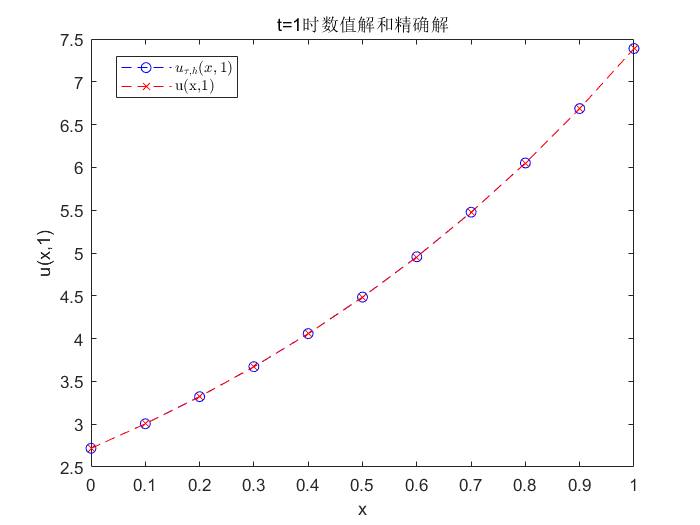
\includegraphics[width=0.7\linewidth]{figures/f1}
	\caption{t=1处的数值解和精确解(向后Euler格式)}
	\label{fig:f1}
\end{figure}

当$\tau=\dfrac{1}{100},h=\dfrac{1}{10}$时,取x=0.5,不同t处的值见表\ref{tab:1},
随着t的增大,误差不断累积,越来越大,
到t=1处误差变得最大。
\begin{table}[htbp]
	\centering
	\caption{x=0.5时,不同t处的数值解、精确解和误差(向后Euler格式)}
	\begin{tabular}{ccccc}
		\toprule[1.5pt]
		k     & t     & 数值解   & 精确解   & 误差 \\
		\midrule[1pt]
		10    & 0.1   & 1.822891  & 1.822119  & 7.7174E-04 \\
		20    & 0.2   & 2.014927  & 2.013753  & 1.1743E-03 \\
		30    & 0.3   & 2.226965  & 2.225541  & 1.4242E-03 \\
		40    & 0.4   & 2.461227  & 2.459603  & 1.6237E-03 \\
		50    & 0.5   & 2.720096  & 2.718282  & 1.8140E-03 \\
		60    & 0.6   & 3.006178  & 3.004166  & 2.0124E-03 \\
		70    & 0.7   & 3.322344  & 3.320117  & 2.2271E-03 \\
		80    & 0.8   & 3.671759  & 3.669297  & 2.4625E-03 \\
		90    & 0.9   & 4.057922  & 4.055200  & 2.7219E-03 \\
		100   & 1     & 4.484697  & 4.481689  & 3.0084E-03 \\
		\bottomrule[1.5pt]
	\end{tabular}%
	\label{tab:1}%
\end{table}%



取不同$\tau$ 和 $h$时,t=1处的误差见图\ref{fig:f2},步长越小,误差也越小。
\begin{figure}
	\centering
	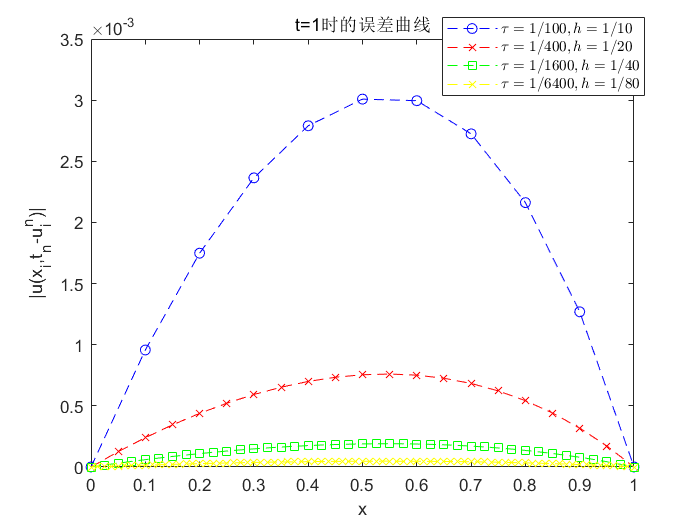
\includegraphics[width=0.7\linewidth]{figures/f2}
	\caption{不同步长下的误差(向后Euler格式)}
	\label{fig:f2}
\end{figure}



取不同步长时,误差和误差比见表\ref{tab:2}, $\tau$变为原来的4倍,$h$变为原来的2倍,误差会变为原来的4倍,
符合$O(\tau+h^2)$的截断误差

% Table generated by Excel2LaTeX from sheet 'Sheet1'
\begin{table}[htbp]
	\centering
	\caption{取不同步长时的误差和误差比(向后Euler格式)}
	\begin{tabular}{ccc}
		\toprule[1.5pt]
		$h,\tau$   & $E_{\infty}(h,\tau)$ & $E_{\infty}(2h,4\tau)/E_{\infty}(h,\tau)$ \\
		\midrule[1pt]
		1/100,1/10 & 3.0084E-03 & * \\
		1/400,1/20 & 7.6035E-04 & 3.956615  \\
		1/1600,1/40 & 1.9023E-04 & 3.997046  \\
		1/6400,1/80 & 4.7566E-05 & 3.999261  \\
		\bottomrule[1.5pt]
	\end{tabular}%
	\label{tab:2}%
\end{table}%

\subsection{Crank-Nicolson格式}
当$\tau=\dfrac{1}{10},h=\dfrac{1}{10}$时,t=1处的数值解和精确解见图\ref{fig:f3},从图像上看很接近。
\begin{figure}
	\centering
	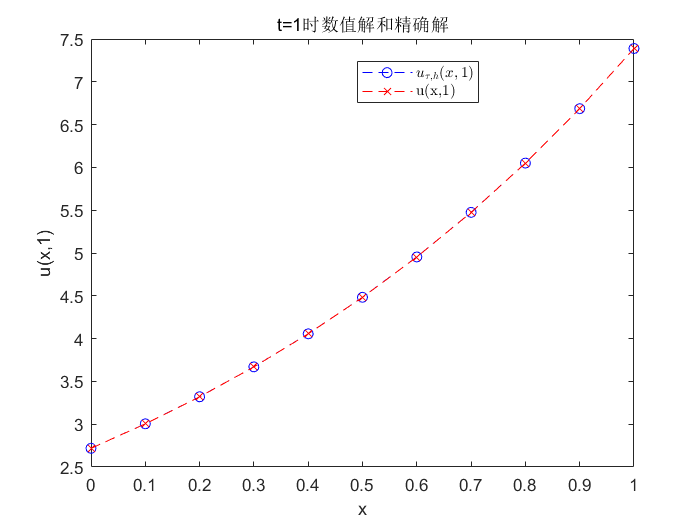
\includegraphics[width=0.7\linewidth]{figures/f3}
	\caption{t=1处的数值解和精确解(Crank-Nicolson格式)}
	\label{fig:f3}
\end{figure}

当$\tau=\dfrac{1}{10},h=\dfrac{1}{10}$时,取x=0.5,不同t处的值见表\ref{tab:3},
当层数越深时,误差越大,这是因为,每一次由k层求解k+1层时都有误差,随着t的增大,误差不断累积,越来越大,
到t=1处误差变得最大。
% Table generated by Excel2LaTeX from sheet 'Sheet1'
% Table generated by Excel2LaTeX from sheet 'Sheet1'
\begin{table}[htbp]
	\centering
	\caption{x=0.5时,不同t处的数值解、精确解和误差(Crank-Nicolson格式)}
	\begin{tabular}{ccccc}
		\toprule[1.5pt]
		k     & t     & 数值解   & 精确解   & 误差 \\
		\midrule[1pt]
		1     & 0.1   & 1.822349  & 1.822119  & 2.3053E-04 \\
		2     & 0.2   & 2.014105  & 2.013753  & 3.5224E-04 \\
		3     & 0.3   & 2.225953  & 2.225541  & 4.1241E-04 \\
		4     & 0.4   & 2.460072  & 2.459603  & 4.6922E-04 \\
		5     & 0.5   & 2.718802  & 2.718282  & 5.2042E-04 \\
		6     & 0.6   & 3.004743  & 3.004166  & 5.7700E-04 \\
		7     & 0.7   & 3.320755  & 3.320117  & 6.3794E-04 \\
		8     & 0.8   & 3.670002  & 3.669297  & 7.0507E-04 \\
		9     & 0.9   & 4.055979  & 4.055200  & 7.7949E-04 \\
		10    & 1     & 4.482550  & 4.481689  & 8.6123E-04 \\
		\bottomrule[1.5pt]
	\end{tabular}%
	\label{tab:3}%
\end{table}%


取不同$\tau$ 和 $h$时,t=1处的误差见图\ref{fig:f4},步长越小,误差也越小。
\begin{figure}
	\centering
	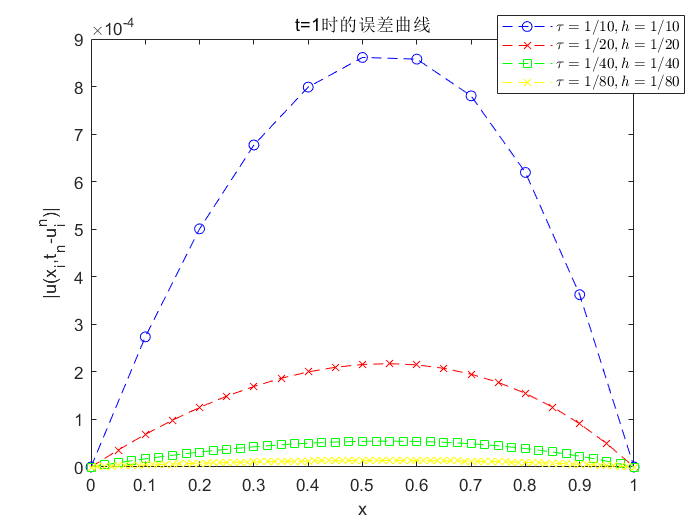
\includegraphics[width=0.7\linewidth]{figures/f4}
	\caption{不同步长下的误差(Crank-Nicolson格式)}
	\label{fig:f4}
\end{figure}


使用Crank-Nicolson格式求数值解,取不同步长时最大误差和最大误差的比值见表\ref{tab:4},	 $\tau$变为原来的2倍,$h$变为原来的2倍,误差会变为原来的4倍,
符合$O(\tau^2+h^2)$的截断误差。

% Table generated by Excel2LaTeX from sheet 'Sheet1'
% Table generated by Excel2LaTeX from sheet 'Sheet1'
\begin{table}[htbp]
	\centering
	\caption{不同步长的最大误差和最大误差的比(Crank-Nicolson格式)}
	\begin{tabular}{ccc}
		\toprule[1.5pt]
		$h,\tau$   & $E_{\infty}(h,\tau)$ & $E_{\infty}(2h,2\tau)/E_{\infty}(h,\tau)$  \\
		\midrule[1pt]
		1/10,1/10 & 8.61E-04 & *    \\
		1/20,1/20 & 2.17E-04 & 3.962274  \\
		1/40,1/40 & 5.44E-05 & 3.998647   \\
		1/80,1/80 & 1.36E-05 & 3.999657   \\
		\bottomrule[1.5pt]
	\end{tabular}%
	\label{tab:4}%
\end{table}%
\subsection{二阶BDF差分格式}
当$\tau=\dfrac{1}{10},h=\dfrac{1}{10}$时,t=1处的数值解和精确解见图\ref{fig:f5},从图像上看很接近。
\begin{figure}
	\centering
	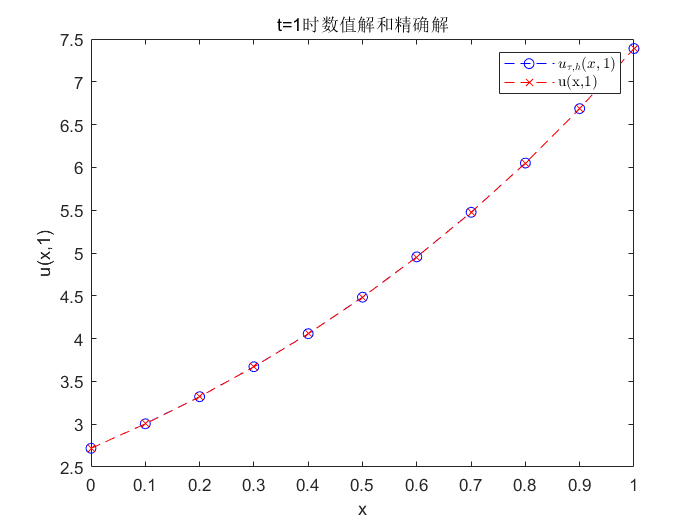
\includegraphics[width=0.7\linewidth]{figures/f5}
	\caption{t=1处的数值解和精确解(二阶BDF差分格式)}
	\label{fig:f5}
\end{figure}

当$\tau=\dfrac{1}{10},h=\dfrac{1}{10}$时,取x=0.5,不同t处的值见表\ref{tab:5}。
% Table generated by Excel2LaTeX from sheet 'Sheet1'
% Table generated by Excel2LaTeX from sheet 'Sheet1'
\begin{table}[htbp]
	\centering
	\caption{x=0.5时,不同t处的数值解、精确解和误差(二阶BDF差分格式)}
	\begin{tabular}{ccccc}
		\toprule[1.5pt]
		k     & t     & 数值解   & 精确解   & 误差 \\
		\midrule[1pt]
		1     & 0.1   & 1.827620  & 1.822119  & 5.50E-03 \\
		2     & 0.2   & 2.018779  & 2.013753  & 5.03E-03 \\
		3     & 0.3   & 2.228923  & 2.225541  & 3.38E-03 \\
		4     & 0.4   & 2.461791  & 2.459603  & 2.19E-03 \\
		5     & 0.5   & 2.719898  & 2.718282  & 1.62E-03 \\
		6     & 0.6   & 3.005622  & 3.004166  & 1.46E-03 \\
		7     & 0.7   & 3.321620  & 3.320117  & 1.50E-03 \\
		8     & 0.8   & 3.670940  & 3.669297  & 1.64E-03 \\
		9     & 0.9   & 4.057022  & 4.055200  & 1.82E-03 \\
		10    & 1     & 4.483712  & 4.481689  & 2.02E-03 \\
		\bottomrule[1.5pt]
	\end{tabular}%
	\label{tab:5}%
\end{table}%

取不同$\tau$ 和 $h$时,t=1处的误差见图\ref{fig:f6},步长越小,误差也越小。
\begin{figure}
	\centering
	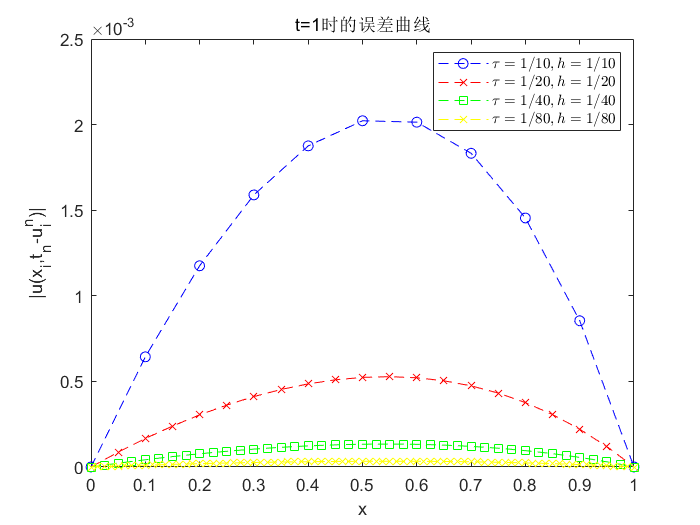
\includegraphics[width=0.7\linewidth]{figures/f6}
	\caption{不同步长下的误差(二阶BDF差分格式)}
	\label{fig:f6}
\end{figure}

取不同步长时,误差和误差比见表\ref{tab:6}, $\tau$变为原来的2倍,$h$变为原来的2倍,误差变为原来的2到3倍,这是因为,虽然$ k \geq 2 $时,截断误差为$O(\tau^2+h^2)$,但是$ k=1 $时,截断误差为$O(\tau+h^2)$,所以达不到4倍。

% Table generated by Excel2LaTeX from sheet 'Sheet1'
\begin{table}[htbp]
	\centering
	\caption{取不同步长时的误差和误差比(二阶BDF差分格式)}
	\begin{tabular}{ccc}
		\toprule[1.5pt]
		$h,\tau$   & $E_{\infty}(h,\tau)$ & $E_{\infty}(2h,4\tau)/E_{\infty}(h,\tau)$ \\
		\midrule[1pt]
	    1/10,1/10 & 5.61E-03 & \multicolumn{1}{c}{*} \\
		1/20,1/20 & 1.90E-03 & 2.9544  \\
		1/40,1/40 & 6.18E-04 & 3.0719  \\
		1/80,1/80 & 1.81E-04 & 3.4202  \\
		\bottomrule[1.5pt]
	\end{tabular}%
	\label{tab:6}%
\end{table}%

\section{总结}
本文建立了三种一维抛物型方程差分格式:向后Euler格式、Crank-Nicolson格式和二阶BDF格式。并运用这三种格式,通过编写matlab程序,对具体的算例进行了数值求解。向后Euler格式的截断误差为  $ O(\tau +h^2) $,Crank-Nicolson格式的截断误差为$ O(\tau^2 +h^2) $,而二阶BDF格式的截断误差则分为两段:当$ k=1 $时,截断误差为$O(\tau+h^2)$,当$ k \geq 2 $时,截断误差为$O(\tau^2+h^2)$,精度为:Crank-Nicolson格式 >二阶BDF格式>向后Euler格式.

%参考文献
\newpage
\begin{thebibliography}{9}%宽度9
	\bibitem[1]{1}
	李荣华. 偏微分方程数值解法[M]. 高等教育出版社, 2005.
	\bibitem[2]{2}
	孙志忠, 计算数学. 偏微分方程数值解法[M]. 科学出版社, 2005.
\end{thebibliography}

\newpage
%附录
\begin{appendices}
	\section{程序流程图}
	程序的流程见图\ref{fig:process}
	\begin{figure}[htbp]
		\centering
		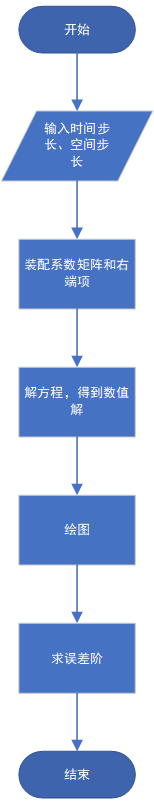
\includegraphics[width=0.2\linewidth]{figures/process}
		\caption{程序流程图}
		\label{fig:process}
	\end{figure}
	
	\section{向后Euler格式代码}
		fa.m 求精确解
		\begin{lstlisting}[language=matlab]
		function r =fa(t,x)
		%  求精确解
		%  @t 时间向量
		%  @x 空间向量
		[t,x]=meshgrid(t,x);
		t=t';
		x=x';
		r=exp(x+t);
		end
		\end{lstlisting}
		
		
		fsolve.m 用向后Euler格式求数值解
		\begin{lstlisting}[language=matlab]
		function [t,x,u] = fsolve(tau,h)
		%   用向后Euler法解抛物方程
		%   @t 时间向量
		%   @x 空间向量
		%   @tau 时间步长
		%   @h 空间步长
		%   @u 数值解
		N=1/tau;%t被分割的区间数
		M=1/h;%x被分割的区间数
		t=0:tau:1;
		x=0:h:1;
		u=ones(N+1,M+1);
		u(1,:)=exp(x);%初值
		%边值
		u(:,1)=exp(t);
		u(:,M+1)=exp(1+t);
		
		r=tau/h^2;%步长系数
		a=ones(M-2,1)*(-r);%下对角线
		c=ones(M-2,1)*(-r);%上对角线
		b=ones(M-1,1)*(1+2*r);%主队角线
		A=diag(b,0)+diag(a,-1)+diag(c,1);%系数矩阵
		for k=2:N+1
		%右端项
		f=u(k-1,2:M);
		f(1)=f(1)+r*u(k,1);
		f(M-1)=f(M-1)+r*u(k,M+1);
		u(k,2:M)=(A\f')';%由k-1层求第k层的值
		end
		end
		\end{lstlisting}
		
		fig.m 绘制误差图,精确解和数值解对比图
		\begin{lstlisting}[language=matlab]
		clc;clear;
		tau=[1/100,1/400,1/1600,1/6400];%时间步长
		h=[1/10,1/20,1/40,1/80];%空间步长
		K=size(tau,2);
		t_cell=cell(K,1);%时间向量
		x_cell=cell(K,1);%空间向量
		u_cell=cell(K,1);%数值解
		ua_cell=cell(K,1);%精确解
		epsilon_cell=cell(K,1);%绝对误差
		for n=1:K
		[t_cell{n,1},x_cell{n,1},u_cell{n,1}]=fsolve(tau(n),h(n));%求数值解
		ua_cell{n,1}=fa(t_cell{n,1},x_cell{n,1});%精确解
		epsilon_cell{n,1}=abs(ua_cell{n,1}-u_cell{n,1});%求绝对误差
		end
		figure(1);
		%t=1,tau=1/100,h=1/10时数值解和精确解对比
		plot(x_cell{1,1},u_cell{1,1}(1/tau(1)+1,:),'b--o'...
		,x_cell{1,1},ua_cell{1,1}(1/tau(1)+1,:),'r--x')
		h=legend('$u_{\tau,h}(x,1)$','u(x,1)');
		set(h,'Interpreter','latex') %设置legend为latex解释器
		title('t=1时数值解和精确解');
		xlabel('x');ylabel('u(x,1)');
		
		%绘制t=1时的误差曲线
		figure(2)
		plot(x_cell{1,1},epsilon_cell{1,1}(1/tau(1)+1,:),'b--o');
		hold on;
		plot(x_cell{2,1},epsilon_cell{2,1}(1/tau(2)+1,:),'r--x');
		hold on;
		plot(x_cell{3,1},epsilon_cell{3,1}(1/tau(3)+1,:),'g--s');
		hold on;
		plot(x_cell{4,1},epsilon_cell{4,1}(1/tau(4)+1,:),'y--x');
		hold on;
		h=legend('$\tau=1/100,h=1/10$','$\tau=1/400,h=1/20$','$\tau=1/1600,h=1/40$','$\tau=1/6400,h=1/80$');
		set(h,'Interpreter','latex') %设置legend为latex解释器
		title('t=1时的误差曲线');
		xlabel('x');ylabel('|u(x_{i},t_{n}-u_{i}^{n})|');
		\end{lstlisting}
		
		data.m 求特定点的数值解,误差分析。
		\begin{lstlisting}[language=matlab]
		clc;clear;
		tao=[1/100,1/400,1/1600,1/6400];%时间步长
		h=[1/10,1/20,1/40,1/80];%空间步长
		K=size(tao,2);
		t_cell=cell(K,1);%时间向量
		x_cell=cell(K,1);%空间向量
		u_cell=cell(K,1);%数值解
		ua_cell=cell(K,1);%精确解
		epsilon_cell=cell(K,1);%绝对误差
		max_epsilon=ones(K,1);
		rate=ones(3,1);%误差比
		for n=1:K
		[t_cell{n,1},x_cell{n,1},u_cell{n,1}]=fsolve(tao(n),h(n));%求数值解
		ua_cell{n,1}=fa(t_cell{n,1},x_cell{n,1});%精确解
		epsilon_cell{n,1}=abs(ua_cell{n,1}-u_cell{n,1});%求绝对误差
		max_epsilon(n,1)=max(epsilon_cell{n,1}(:));%求最大误差
		end
		
		%E(t,h)/E(4t,2h)
		for n=1:K-1
		rate(n,1)=max_epsilon(n,1)/max_epsilon(n+1,1);
		end
		
		%当x=0.5时,取t=0.1,0.2,...1时,误差的变化,tao=1/100,h=1/10;
		u_1=ones(10,1);%特定点数值解
		ua_1=ones(10,1);%特定点精确解
		[t,x,u]=fsolve(tao(1),h(1));
		ua=fa(t,x);
		u_1=u(11:10:101,6);
		ua_1=ua(11:10:101,6);
		epsion_1=abs(u_1-ua_1);%误差
		\end{lstlisting}
	\section{Crank-Nicolson格式代码}
	fa.m 求精确解:与向后Euler格式相同
	
	fsolve.m 用Crank-Nicolson格式求数值解
	\begin{lstlisting}[language=matlab]
	function [t,x,u] = fsolve(tau,h)
	%   用Crank-Nicolson格式解求数值解
	%   @t 时间向量
	%   @x 空间向量
	%   @tau 时间步长
	%   @h 空间步长
	%   @u 数值解
	N=1/tau;%t被分割的区间数
	M=1/h;%x被分割的区间数
	t=0:tau:1;
	x=0:h:1;
	u=ones(N+1,M+1);
	u(1,:)=exp(x);%初值
	%边值
	u(:,1)=exp(t);
	u(:,M+1)=exp(1+t);
	
	r=tau/h^2;%步长系数
	a1=ones(M-2,1)*(-r/2);%下对角线
	b1=ones(M-1,1)*(1+r);%主队角线
	c1=ones(M-2,1)*(-r/2);%上对角线
	A1=diag(b1,0)+diag(a1,-1)+diag(c1,1);%系数矩阵
	
	a2=-a1;
	b2=ones(M-1,1)*(1-r);
	c2=-c1;
	A2=diag(b2,0)+diag(a2,-1)+diag(c2,1);%系数矩阵
	for k=2:N+1
	%右端项
	f=A2*u(k-1,2:M)';
	f(1)=f(1)+r/2*(u(k,1)+u(k-1,1));
	f(M-1)=f(M-1)+r/2*(u(k,M+1)+u(k-1,M+1));
	u(k,2:M)=(A1\f)';%由k-1层求第k层的值
	end
	end
	\end{lstlisting}
	
	fig.m 绘制误差图,精确解和数值解对比图
	\begin{lstlisting}[language=matlab]
	clc;clear;
	tau=[1/10,1/20,1/40,1/80];%时间步长
	h=[1/10,1/20,1/40,1/80];%空间步长
	K=size(tau,2);
	t_cell=cell(K,1);%时间向量
	x_cell=cell(K,1);%空间向量
	u_cell=cell(K,1);%数值解
	ua_cell=cell(K,1);%精确解
	epsilon_cell=cell(K,1);%绝对误差
	for n=1:K
	[t_cell{n,1},x_cell{n,1},u_cell{n,1}]=fsolve(tau(n),h(n));%求数值解
	ua_cell{n,1}=fa(t_cell{n,1},x_cell{n,1});%精确解
	epsilon_cell{n,1}=abs(ua_cell{n,1}-u_cell{n,1});%求绝对误差
	end
	figure(1);
	%t=1,tau=1/100,h=1/10时数值解和精确解对比
	plot(x_cell{1,1},u_cell{1,1}(1/tau(1)+1,:),'b--o'...
	,x_cell{1,1},ua_cell{1,1}(1/tau(1)+1,:),'r--x')
	h=legend('$u_{\tau,h}(x,1)$','u(x,1)');
	set(h,'Interpreter','latex') %设置legend为latex解释器
	title('t=1时数值解和精确解');
	xlabel('x');ylabel('u(x,1)');
	
	%绘制t=1时的误差曲线
	figure(2)
	plot(x_cell{1,1},epsilon_cell{1,1}(1/tau(1)+1,:),'b--o');
	hold on;
	plot(x_cell{2,1},epsilon_cell{2,1}(1/tau(2)+1,:),'r--x');
	hold on;
	plot(x_cell{3,1},epsilon_cell{3,1}(1/tau(3)+1,:),'g--s');
	hold on;
	plot(x_cell{4,1},epsilon_cell{4,1}(1/tau(4)+1,:),'y--x');
	hold on;
	h=legend('$\tau=1/10,h=1/10$','$\tau=1/20,h=1/20$','$\tau=1/40,h=1/40$','$\tau=1/80,h=1/80$');
	set(h,'Interpreter','latex') %设置legend为latex解释器
	title('t=1时的误差曲线');
	xlabel('x');ylabel('|u(x_{i},t_{n}-u_{i}^{n})|');
	\end{lstlisting}
	
	data.m 求特定点的数值解,误差分析。
	\begin{lstlisting}[language=matlab]
	clc;clear;
	tau=[1/10,1/20,1/40,1/80];%时间步长
	h=[1/10,1/20,1/40,1/80];%空间步长
	K=size(tau,2);
	t_cell=cell(K,1);%时间向量
	x_cell=cell(K,1);%空间向量
	u_cell=cell(K,1);%数值解
	ua_cell=cell(K,1);%精确解
	epsilon_cell=cell(K,1);%绝对误差
	max_epsilon=ones(K,1);
	rate=ones(3,1);%误差比
	for n=1:K
	[t_cell{n,1},x_cell{n,1},u_cell{n,1}]=fsolve(tau(n),h(n));%求数值解
	ua_cell{n,1}=fa(t_cell{n,1},x_cell{n,1});%精确解
	epsilon_cell{n,1}=abs(ua_cell{n,1}-u_cell{n,1});%求绝对误差
	max_epsilon(n,1)=max(epsilon_cell{n,1}(:));%求最大误差
	end
	
	%E(t,h)/E(2t,2h)
	for n=1:K-1
	rate(n,1)=max_epsilon(n,1)/max_epsilon(n+1,1);
	end
	
	%当x=0.5时,取t=0.1,0.2,...1时,误差的变化(tau=1/10,h=1/10);
	u_1=zeros(10,1);%特定点数值解
	ua_1=zeros(10,1);%特定点精确解
	[t,x,u]=fsolve(tau(1),h(1));
	ua=fa(t,x);
	u_1=u(2:1:11,1/h(1)/2+1);
	ua_1=ua(2:1:11,1/h(1)/2+1);
	epsion_1=abs(u_1-ua_1);%误差
	\end{lstlisting}
	
	\section{二阶BDF格式代码}
	fa.m 求精确解,与前面相同
	
	fig.m 绘制误差图,精确解和数值解对比图,与Crank-Nicolson格式相同
	
	data.m 求特定点的数值解,误差分析,与Crank-Nicolson格式相同
	
	fsolve.m 用BDF格式求数值解
	\begin{lstlisting}[language=matlab]
	function [t,x,u] = fsolve(tau,h)
	%   用BDF格式解抛物方程
	%   @t 时间向量
	%   @x 空间向量
	%   @tau 时间步长
	%   @h 空间步长
	%   @u 数值解
	N=1/tau;%t被分割的区间数
	M=1/h;%x被分割的区间数
	t=0:tau:1;
	x=0:h:1;
	u=ones(N+1,M+1);
	u(1,:)=exp(x);%初值
	%边值
	u(:,1)=exp(t);
	u(:,M+1)=exp(1+t);
	
	r=tau/h^2;%步长系数
	a=ones(M-2,1)*(-r);%下对角线
	c=ones(M-2,1)*(-r);%上对角线
	b=ones(M-1,1)*(1+2*r);%主队角线
	A1=diag(b,0)+diag(a,-1)+diag(c,1);%向后Euer法系数矩阵
	
	a=ones(M-2,1)*(r);%下对角线
	c=ones(M-2,1)*(r);%上对角线
	b=ones(M-1,1)*(-(2*r+3/2));%主队角线
	A2=diag(b,0)+diag(a,-1)+diag(c,1);%向后Euer法系数矩阵
	
	%由第0层求第1层
	f=u(1,2:M);
	f(1)=f(1)+r*u(2,1);
	f(M-1)=f(M-1)+r*u(2,M+1);
	u(2,2:M)=(A1\f')';%由0层求第1层的值
	
	%用Crank-Nicolson格式求出的第1层替代向后Euler法求出的第一层数值解
	%     [t2,x2,u2]=fsolve12(tau,h);
	%     u(2,2:M)=u2(2,2:M);
	
	%第2层到N层
	for k=3:N+1
	%右端项
	F=-2*u(k-1,2:M)+1/2*u(k-2,2:M);
	F(1)=F(1)-r*u(k,1);
	F(M-1)=F(M-1)-r*u(k,M+1);
	u(k,2:M)=(A2\F')';%由k-1层求第k层的值
	end
	end
	\end{lstlisting}
\end{appendices}

\end{document}